\section{Imaging and Image Processing}

Considering prediction of brain activity requires that we look not only at the
current state of brain simulation, but also towards the future. A biological
brain processing the life of an organism, and a simulation of the same requires
a link to made between the two: the state of the brain must be copied over as a
snapshot. This imaging process would likely take the form of an in vitro scan of
a preserved nervous system or some form of in vivo scan. These images would be
processed and turned into a model that could be simulated. Current techniques for imaging the brain give us some insight to how this
uploading process might function and perform.

\subsection{Current Methods of Scanning the brain}

Given a 2D substrate such as a layer of brain tissue, there are several methods
of producing a high resolution image. These methods must balance the resolution
and noise levels required of model creation, with the speed with which the image
is taken \autocite{bostrom_whole_2008,mikula_progress_2016}.

\begin{figure}[h]
    \centering
    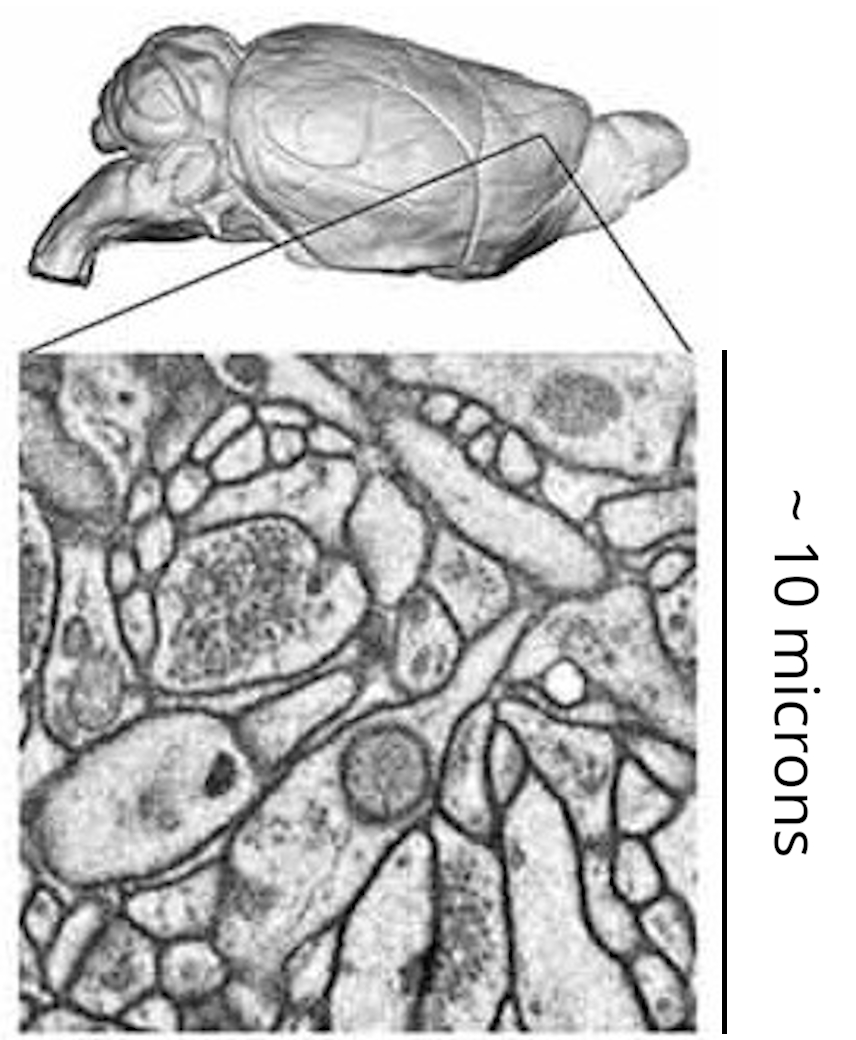
\includegraphics[scale=2]{figures/images/enlarge.jpg}
    \DoubleCaption{Illustration of the scale of neurons in the brain.}
    {Adapted from \cite[fig. 1]{mikula_progress_2016}}
    \label{scaleexample}
\end{figure}
\vspace{1ex}

Given the level of emulation that is intended from a model, the images that
synthesise the model must resolve a minimum level of detail. In figure
\ref{scaleexample}, the general position of neuron somas and the rough links
between them can be identified, but more subtle morphologies of these links are
missing. Perhaps another imaging method could resolve further detail. The
specifications and drawbacks of several imaging methods are described below.

\subsubsection*{MRI}

Magnetic Resonance Imaging (MRI) scanning is a common medical procedure, but at
current generally available resolutions is not suitable for reconstructing any
kind of neural model owing to its low resolution. Future technologies that which
to enable brain emulation of the biologically alive would need to offer a
similar feature set as MRI scanning while producing images many thousands of
times more detailed. Such MRI microscopy does exist currently, but is
significantly more limited in scale, scanning small chunks of cortical tissue at
a very high resolution
\autocite{johnson_three-dimensional_1987,bostrom_whole_2008}.

\subsubsection*{Electron Microscope Scanning}

TODO

In order to reach the required resolutions today, Electron Microscopes (EM) are
commonly used. 

- Very precise
- Can take a very long time
- Need well "frozen" slices of the brain for this to be of any use or you'll
have major measurement drift as the brain decays.

\subsection{Turning image data into a connectome}
TODO:
\begin{quote}
    Dense connectomic mapping of neuronal circuits is limited by the time and
    effort required to analyse 3D electron microscopy (EM) datasets. Algorithms
    designed to automate image segmentation suffer from substantial error rates
    and require significant manual error correction. Any improvement in
    segmentation error rates would therefore directly reduce the time required
    to analyse 3D EM data.
    \autocite{pallotto_extracellular_2015} \autocite{tomsett_virtual_2015}

    \begin{figure}[h]
        \centering
        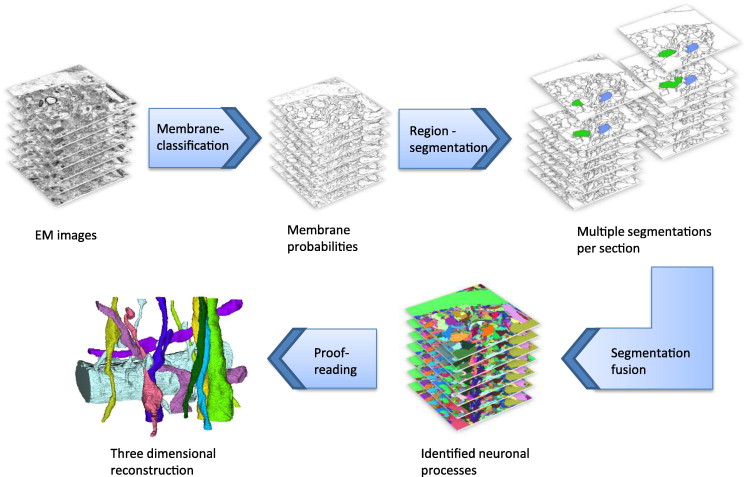
\includegraphics[scale=0.75]{figures/images/reconstruction.jpg}
        \DoubleCaption{Illustration of a typical workflow for connectome
        reconstruction}
        {Reproduced from \cite{kaynig_large-scale_2015}}
        \label{reconstruction}
    \end{figure}
    \vspace{1ex}

    The delineation of morphologies has proven to be the most difficult step to
    automate. Current machine learning-based analysis methods enable
    semi-automated reconstructions (segmentations) of neurons that still require
    significant human effort to correct.
    \autocite{helmstaedter_connectomic_2013}
\end{quote}

\subsection[Error induced through noise]{Examination of Error induced through the imaging process}

Prediction of future brain activity through simulation requires an accurate and
detailed connectome of a brain, with synapses and neurons correctly located in
space.\autocite{bostrom_whole_2008} The accuracy of such a model depends on the
resolution of the imaging method used to create it. The error resulting from
such a imaging method is the measurement error. Depending on imaging procedure, brain matter may shift in composition during the course of the scan, which is the cause of measurement drift, itself a form of measurement error.

\setlength{\tabcolsep}{4ex}
\renewcommand{\arraystretch}{1.1}
\begin{table}[ht]
    \centering
    \begin{tabular}{@{}llll@{}}
        Method              & Resolution                 & Time    & Error(approx.) \\
        \hline
        MRI                 & 6$\mu m$                   & 30mins  & 95\%           \\
        MRI microscopy      & 3$\mu m$                   & -       & 85\%           \\
        XRay microscopy     & 30nm                       & -       & 30\%           \\
        Electron microscopy & \textasciitilde 30nm-0.1nm & >3mnths & <1\%           \\
        Theoretical Ideal   & <5nm                       & <500s   & <1\%           \\
        \hline
    \end{tabular}
    \DoubleCaption{Comparison of imaging methods.}{Error approximated from size of dendritic spines.}
    \label{imagemethodcomparison1}
\end{table}
\setlength{\tabcolsep}{1ex}

